%& -shell-escape

\documentclass[a4paper]{report}

\usepackage[utf8]{inputenc}
\usepackage[francais]{babel}
\usepackage[T1]{fontenc}
\usepackage{amsmath}
\usepackage{amsfonts}
\usepackage{amssymb}
\usepackage{placeins}
\usepackage{listings}
\usepackage{color}
\usepackage{textcomp}

%----- Package français
\usepackage[utf8]{inputenc} %reconnaissance des accents
\usepackage[francais]{babel} %document en français
\usepackage[T1]{fontenc} %codage des fonts TeX ?



%----- math
\usepackage{amsmath}
\usepackage{dsfont}
\usepackage{calrsfs}

%----- images
\usepackage{graphicx}

%----- dot graphs
\usepackage{pgf}
\usepackage{tikz}
\usetikzlibrary{shapes,arrows}
\usepackage[debug]{dot2texi}



\title{Automatic test case generation for java}
%\author{Thomas BRIEN}
%\date{28 janvier 2013}

\begin{document}
%\maketitle
\tableofcontents

\renewcommand{\thesection}{\arabic{section}}

\newtheorem{theorem}{Theorem}
\newtheorem{lemma}{Lemme}

\renewcommand{\thetheorem}{\empty{}}
\renewcommand{\thelemma}{\empty{}} 

\newenvironment{proof}[1][Proof]{\begin{trivlist}
\item[\hskip \labelsep {\bfseries #1}]}{\end{trivlist}}
\newenvironment{definition}[1][Definition]{\begin{trivlist}
\item[\hskip \labelsep {\bfseries #1}]}{\end{trivlist}}
\newenvironment{example}[1][Example]{\begin{trivlist}
\item[\hskip \labelsep {\bfseries #1}]}{\end{trivlist}}
\newenvironment{remark}[1][Rq:]{\begin{trivlist}
\item[\hskip \labelsep {\bfseries #1}]}{\end{trivlist}}
\newenvironment{rappel}[1][rappel:]{\begin{trivlist}
\item[\hskip \labelsep {\bfseries #1}]}{\end{trivlist}}


\chapter*{Introduction}
\addcontentsline{toc}{chapter}{Introduction}




\chapter*{Plate-forme cible}
\addcontentsline{toc}{chapter}{Plate-forme cible}




\chapter*{État de l'art}
\addcontentsline{toc}{chapter}{État de l'art}


\section*{Les tests classiques, avec JUnit}
\addcontentsline{toc}{section}{Les tests classiques, avec JUnit}

\subsection*{Tests unitaires}
\addcontentsline{toc}{subsection}{Tests unitaires}
Les tests unitaires ont pour but de prouver la validité d'un objet. Par exemple, on souhaite parcourir la totalité du code en lançant le programme avec des valeurs clef choisies par le programmeur chargé des tests.

\subsection*{Tests d'intégration}
\addcontentsline{toc}{subsection}{Tests d'intégration}
Les tests d'intégration visent à valider la bonne interaction entre plusieurs composants du système.

\subsection*{Tests système}
\addcontentsline{toc}{subsection}{Tests système}
Comme on peut s'en douter, les tests système permettent de contrôler le système dans son ensemble.

\section*{Les tests par contrat}
\addcontentsline{toc}{section}{Les tests par contrat}
L'introduction de contrats dans le code permet de définir les conditions de début, de fin, et les constantes d'exécution.
\section*{Les tests par mutation}
\addcontentsline{toc}{section}{Les tests par mutation}

\section*{Les méthodes de test automatique}
\addcontentsline{toc}{section}{Les méthodes de test automatique}
- IOCO théorie\\
- ioLTS\\
- FSM/EFSM (Extended Finit State Machin)\\
- MBT (Model-Based Testing)\\





\chapter*{Idées et mise en œuvre}
\addcontentsline{toc}{chapter}{Idées et mise en œuvre}
- random testing\\
- dynamic path construction leaded by coverage (récursive)\\
- logic modelisation (FOL) and SMT solver\\

On raisonne sur le code source, et plus particulièrement sur des blocs de code. A partir de ce point, nous appellerons fonction élémentaire une partie de code dont la séquence d'exécution ne dépend d'aucune variable. Plus précisément, dans notre cas, un code java qui ne contient pas d'accolades.\\
\newline
Par exemple, le code java suivant contient deux actions elementaires: val=arg1 et val+=arg2\\

\begin{lstlisting}
public int exemple(int arg1, int arg2){
		int val = 0;
		if(this.a<arg1){
			val = arg1;
		}
		if(val<arg2){
			val += arg2;
		}
		return val;
	}
\end{lstlisting}
A cette fonction, on associera le graph suivant:\\


\begin{dot2tex}[dot, tikz,options=-tmath --autosize]
digraph G {

rankdir=LR;

node [shape="none"]; start;

node [shape="circle",color="black"]; a_0 a_1 a_2 a_3;
node [shape="diamond", color="black"]; d_0 d_1 d_2;
node [shape="circle",peripheries=2, style="filled", color="black"]; o_0 o_1 o_2 o_3;

start -> a_0;
a_0 -> d_0;
d_0 -> a_1;
d_0 -> d_1;
a_1 -> d_2;
d_1 -> a_2;
d_1 -> o_0;
a_2 -> o_1;
d_2 -> o_2;
d_2 -> a_3;
a_3 -> o_3;
}
\end{dot2tex}

\begin{figure}[position]
   \caption{\label{étiquette} titre}
   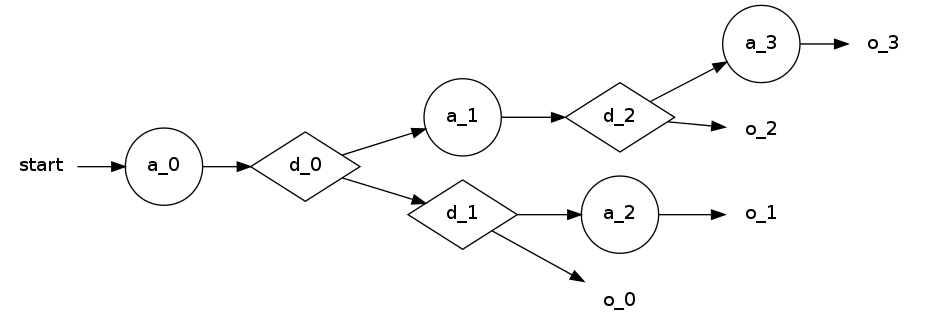
\includegraphics[scale=0.4]{../graphviz/doubleStackGraph.png}
\end{figure}
%\newline



En suivant notre modélisation, on obtient deux actions élémentaires:


\chapter*{Réalisations}
\addcontentsline{toc}{chapter}{Réalisations}


\chapter*{Bibliographie}
\addcontentsline{toc}{chapter}{Bibliographie}
\section*{BDD}
\addcontentsline{toc}{section}{BDD}

\section*{Les tests par mutation}
\addcontentsline{toc}{section}{Les tests par mutation}

\section*{Automatisation}
\addcontentsline{toc}{section}{Automatisation}

$[3.1]$ Bertrand Meyer, Ilinca Ciupa, Andreas Leitner and Lisa (Ling) Liu, \textit{Automatic Testing of Object-Oriented Software}, in SOFSEM 2007\\
$[3.2]$ Hans-Gerhard Gross and Arjan Seesing, 
\textit{A Genetic Programming Approach to Automated Test Generation for Object Oriented Software}, Report TUD-SERG-2006-017


\end{document}